\section{Propiedades matemáticas y optimización}\label{sec:propiedades}

Esta sección analiza la estructura diferencial, convexa, de optimalidad y de robustez del problema \eqref{eq:objetivo_smcfhr}. Las demostraciones completas de los resultados enunciados se presentan en el Apéndice~\ref{ap:demos}, manteniendo aquí la derivación del gradiente, los teoremas centrales y sus consecuencias prácticas.

\subsection{Estructura diferencial, gradiente analítico y L-BFGS-B}

La derivada de la pérdida de Huber $\rho_\delta(r)$ es la función de influencia acotada $\psi_\delta : \mathbb{R} \to [-\delta, \delta]$,
\begin{equation}
\psi_\delta(r) := \rho_\delta'(r) = \begin{cases}
r & \text{si } |r| \le \delta, \\
\delta\,\sign(r) & \text{si } |r| > \delta,
\end{cases}
\label{eq:psi_huber}
\end{equation}
que es continua en todo $\mathbb{R}$ y globalmente Lipschitz con constante $1$. Definiendo el vector de residuos estandarizados $\mathbf{r}(b, \mathbf{w}) := \tilde{\mathbf{y}} - b\mathbf{1}_n - Z\mathbf{w} \in \mathbb{R}^n$ y aplicando la regla de la cadena sobre $J(b,\mathbf{w})$ en \eqref{eq:objetivo_smcfhr}, las derivadas parciales exactas respecto al intercepto y los pesos son:
\begin{equation}
\frac{\partial J}{\partial b}(b,\mathbf{w}) = -\frac{1}{n}\sum_{k=1}^{n} \psi_\delta(r_k), \qquad
\nabla_{\mathbf{w}} J(b,\mathbf{w}) = -\frac{1}{n} Z^\top \psi_\delta(\mathbf{r}) + D_\alpha \mathbf{w},
\label{eq:gradiente_smcfhr}
\end{equation}
donde $\psi_\delta(\mathbf{r})$ se evalúa componente a componente. Estas expresiones coinciden exactamente con el método \texttt{\_objective\_and\_grad\_debug} implementado en el estimador.

Conviene precisar el orden de regularidad de $J$: la función objetivo es continuamente diferenciable ($C^1(\mathbb{R}^{p+1})$) con gradiente Lipschitz continuo, pero \emph{no} es dos veces continuamente diferenciable ($C^2$) en los hiperplanos de transición $|r_k(b,\mathbf{w})| = \delta$. En el interior de cada región abierta donde $|r_k| \ne \delta$ para todo $k$, la matriz Hessiana existe y toma la forma
\begin{equation}
\nabla^2 J(b,\mathbf{w}) = \frac{1}{n} \begin{bmatrix} \mathbf{1}_n^\top \\ Z^\top \end{bmatrix} \diag(\mathbf{1}_{\mathcal{I}_{\mathrm{quad}}}) \begin{bmatrix} \mathbf{1}_n & Z \end{bmatrix} + \begin{bmatrix} 0 & \mathbf{0}^\top \\ \mathbf{0} & D_\alpha \end{bmatrix},
\label{eq:hessiana_regiones}
\end{equation}
donde $\mathcal{I}_{\mathrm{quad}} := \{k \in \{1,\dots,n\} : |r_k| < \delta\}$ es el conjunto de observaciones en régimen cuadrático. Fuera de esos hiperplanos, $\nabla^2 J$ es semidefinida positiva; en los puntos de quiebre $|r_k| = \delta$, la segunda derivada presenta saltos finitos. Esta estructura explica la elección de L-BFGS-B \cite{byrd1995lbfgsb,zhu1997lbfgsb}: al requerir únicamente valores del objetivo, gradientes analíticos de primer orden y proyecciones simples sobre las cotas de caja $\mathbb{R} \times \mathcal{C}$, L-BFGS-B evita la inversión de Hessianas discontinuas y garantiza convergencia hacia puntos estacionarios con costo $O(np)$ por evaluación.

\begin{figure}[!htbp]
\centering
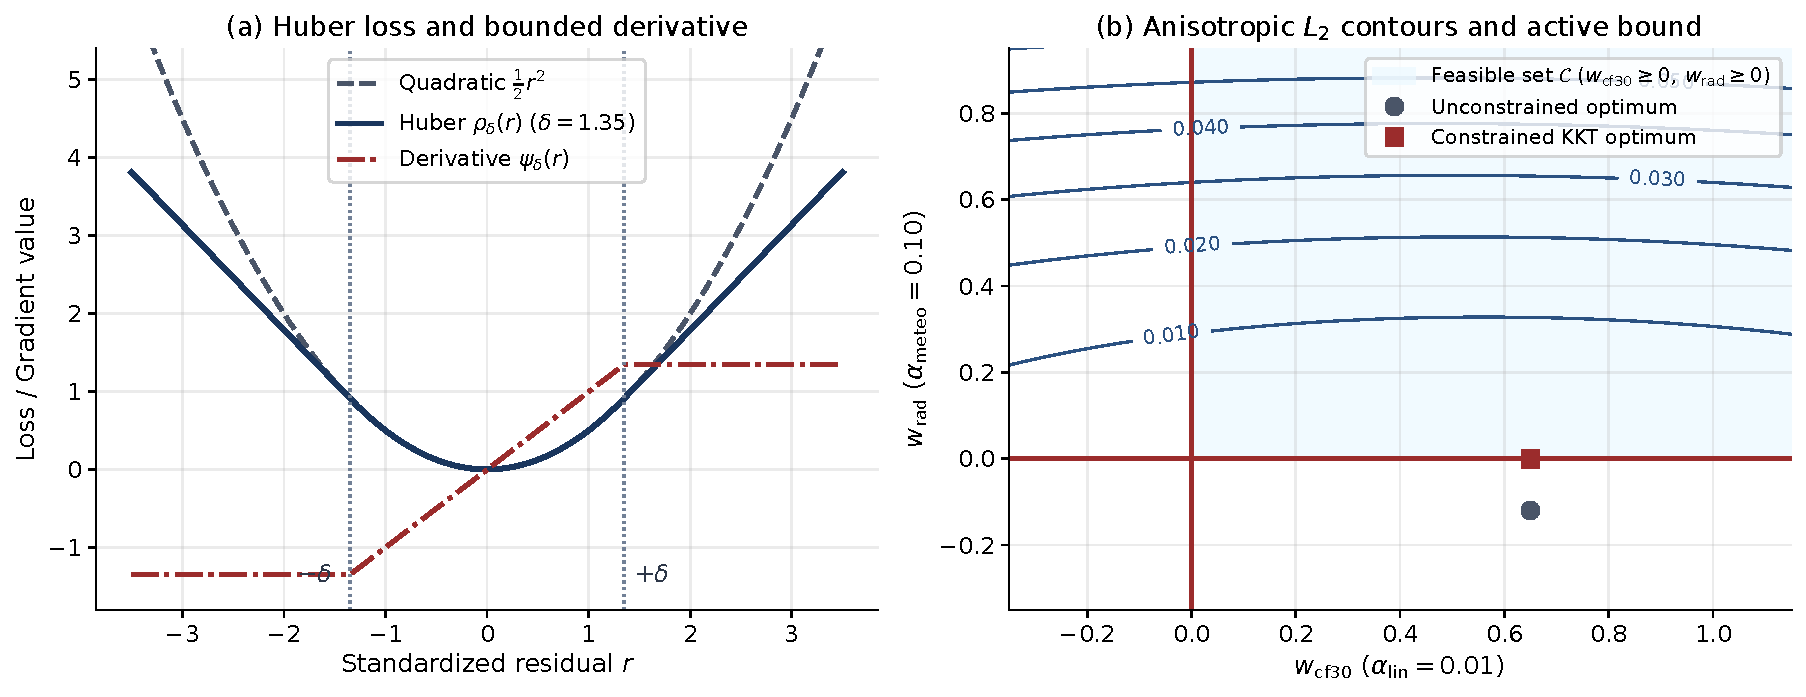
\includegraphics[width=0.98\textwidth]{figures/fig_huber_estructura.pdf}
\caption{Estructura analítica de SM-CFHR: (a) pérdida de Huber $\rho_\delta(r)$ frente a la pérdida cuadrática y función de influencia acotada $\psi_\delta(r)$ en $\pm\delta = 1{,}35$; (b) curvas de nivel de la penalización $L_2$ anisotrópica ($\alpha_{\mathrm{meteo}} = 10\,\alpha_{\mathrm{lin}}$) y cota activa en la región factible $\mathcal{C}$.}
\label{fig:huber_estructura}
\end{figure}

\subsection{Convexidad, existencia, unicidad y condiciones KKT}

A diferencia de la documentación informal del código, que denomina al problema «estrictamente convexo» sin matices, un análisis riguroso muestra que la convexidad estricta global puede fallar respecto al intercepto $b$. Los siguientes resultados delimitan exactamente qué propiedades se cumplen bajo las hipótesis reales de SM-CFHR.

\begin{theorem}[Convexidad y existencia de soluciones]\label{thm:convexidad_existencia}
Supóngase $\delta > 0$, $\alpha_{\mathrm{lin}} > 0$ y $\alpha_{\mathrm{meteo}} > 0$. Entonces:
\begin{enumerate}
    \item El conjunto factible $\Omega := \mathbb{R} \times \mathcal{C}$ es cerrado y convexo en $\mathbb{R}^{p+1}$.
    \item La función objetivo $J(b,\mathbf{w})$ es convexa y $C^1$ en $\mathbb{R}^{p+1}$, con gradiente globalmente Lipschitz continuo de constante $L_J \le \frac{1}{n}\left\|\begin{bmatrix}\mathbf{1}_n & Z\end{bmatrix}\right\|_2^2 + \max\{\alpha_{\mathrm{lin}}, \alpha_{\mathrm{meteo}}\}$.
    \item $J$ es coerciva sobre $\Omega$ (esto es, $J(b,\mathbf{w}) \to +\infty$ cuando $\|(b,\mathbf{w})\|_2 \to \infty$) y acotada inferiormente por $0$; por consiguiente, existe al menos un minimizador global $(b^*, \mathbf{w}^*) \in \Omega$.
\end{enumerate}
\end{theorem}

La pérdida de Huber $\rho_\delta$ es estrictamente convexa únicamente en el intervalo $[-\delta, \delta]$ y afín fuera de él. En consecuencia, $J(b,\mathbf{w})$ es estrictamente convexa en $\mathbf{w}$ gracias al término $\frac{1}{2}\mathbf{w}^\top D_\alpha \mathbf{w}$ con $D_\alpha \succ 0$, pero \emph{no} es globalmente estrictamente convexa en $(b,\mathbf{w})$. El siguiente resultado precisa cuándo la solución es única.

\begin{theorem}[Unicidad exacta y caso degenerado del intercepto]\label{thm:unicidad}
Bajo las hipótesis del Teorema~\ref{thm:convexidad_existencia}:
\begin{enumerate}
    \item El vector óptimo de coeficientes $\mathbf{w}^* \in \mathcal{C}$ es \textbf{único}.
    \item El conjunto de interceptos óptimos $\mathcal{B}^* := \{b \in \mathbb{R} : (b, \mathbf{w}^*) \text{ minimiza } J \text{ en } \Omega\}$ es un intervalo compacto y convexo. Si existe al menos una observación $k \in \{1,\dots,n\}$ cuyo residuo óptimo satisface $|\tilde{y}_k - b^* - \mathbf{z}_k^\top \mathbf{w}^*| < \delta$ para algún $b^* \in \mathcal{B}^*$, entonces el intercepto óptimo $b^*$ también es \textbf{único}.
    \item En el caso patológico en que $|r_k(b^*,\mathbf{w}^*)| \ge \delta$ para todo $k=1,\dots,n$ (todas las observaciones caen fuera de la banda cuadrática) y $n$ es par con igual número de residuos positivos y negativos, $\mathcal{B}^*$ puede ser un intervalo no degenerado de múltiples interceptos con idéntico valor objetivo.
\end{enumerate}
\end{theorem}

Dado que $\mathcal{C}$ está definido por desigualdades afines y $(0, \mathbf{0})$ pertenece al interior relativo de la región factible (con punto estrictamente interior para las cotas seleccionando $w_j = 1 > 0$ para $j \in \mathcal{M}_+$), se satisface la condición de cualificación de Slater \cite{boyd2004convex}. Por tanto, las condiciones de Karush--Kuhn--Tucker (KKT) son necesarias y suficientes para la optimalidad global.

\begin{proposition}[Condiciones KKT y complementariedad]\label{prop:kkt}
Un punto $(b^*, \mathbf{w}^*) \in \Omega$ es minimizador global de \eqref{eq:objetivo_smcfhr} si y solo si existen multiplicadores $\boldsymbol{\lambda}^* \in \mathbb{R}_{\ge 0}^{|\mathcal{M}_+|}$ tales que:
\begin{align}
\frac{1}{n}\sum_{k=1}^{n} \psi_\delta(r_k^*) &= 0, \label{eq:kkt_b} \\
-\frac{1}{n}\left(Z^\top \psi_\delta(\mathbf{r}^*)\right)_j + d_j w_j^* &= 0 && \forall j \notin \mathcal{M}_+, \label{eq:kkt_free} \\
-\frac{1}{n}\left(Z^\top \psi_\delta(\mathbf{r}^*)\right)_j + d_j w_j^* &= \lambda_j^* \ge 0, \quad w_j^* \ge 0, \quad \lambda_j^* w_j^* = 0 && \forall j \in \mathcal{M}_+. \label{eq:kkt_mono}
\end{align}
En particular, para toda variable restringida $j \in \mathcal{M}_+$ cuya cota esté activa ($w_j^* = 0$), la correlación residual ponderada por Huber satisface $\frac{1}{n}(Z^\top \psi_\delta(\mathbf{r}^*))_j \le 0$.
\end{proposition}

\subsection{Robustez, monotonía parcial y complejidad}

La ecuación \eqref{eq:kkt_b} y el término $\frac{1}{n}Z^\top \psi_\delta(\mathbf{r}^*)$ delimitan con exactitud el alcance de la robustez de SM-CFHR. Como $|\psi_\delta(r_k)| \le \delta$ para todo $r_k \in \mathbb{R}$, la contribución de cualquier observación anómala en la variable respuesta $\tilde{y}_k$ sobre el gradiente está acotada por $\delta/n$ en el intercepto y por $(\delta/n)\|\mathbf{z}_k\|_\infty$ en los coeficientes. Sin embargo, SM-CFHR \emph{no} es robusto frente a puntos de apalancamiento arbitrariamente grandes en el espacio de predictores $\|\mathbf{z}_k\|$, pues el estimador no aplica ponderación acotada sobre $Z$ (tipo Mallows o Schweppe); su diseño asume que las variables de entrada meteorológicas y autorregresivas están acotadas físicamente o imputadas por mediana, mientras que las anomalías severas ocurren principalmente en la generación observada $y_{i,s}$.

Respecto a la interpretabilidad física, para todo predictor restringido $j \in \mathcal{M}_+$, $w_j^* \ge 0$ implica que el predictor latente $\hat{b} + \mathbf{z}^\top \hat{\mathbf{w}}$ es una función monótona no decreciente de $x_j$ cuando se mantienen fijas las demás coordenadas (y $\tilde{s}_j > 0$). Tras aplicar el operador monótono no decreciente $\clip(\cdot, 0, 1)$ y multiplicar por $24\,000\,C_{i,t} H_{\mathrm{dir}} > 0$, la energía predicha $\hat{y}_q$ hereda monotonía parcial no decreciente respecto a $\mathrm{cf}_{30}$ y $\mathrm{rad\_pron}$ (ceteris paribus), y garantiza factibilidad física $\hat{y}_q \in [0, 24\,000\,H_{\mathrm{dir}}\,C_{i,t}]$. No obstante, esta propiedad no equivale a monotonía física universal ante variaciones conjuntas de variables correlacionadas (por ejemplo, si un aumento de radiación coincide con incrementos en temperatura de celda o cambios en las anomalías).

Finalmente, cada evaluación del objetivo y del gradiente requiere dos productos matriz-vector con $Z \in \mathbb{R}^{n \times p}$ y operaciones vectoriales de orden $O(n + p)$, por lo que su complejidad temporal por iteración es $O(np)$ con $p \in \{7, 17\}$, y su complejidad espacial es $O(np + mp)$ para almacenar la matriz estandarizada y los $m$ pares de curvatura recientes de L-BFGS-B (por defecto $m=10$ en SciPy).
